\documentclass{article}
\usepackage{graphicx}  
\usepackage[landscape]{geometry}
%\usepackage[pdftex]{color}
\usepackage[dvipdfm]{color}


\usepackage{url}
\usepackage{multicol}
\usepackage{amsmath}
\usepackage{amsfonts}
\newcommand{\ex}{\color{blue}}
\pagestyle{empty}
\advance\topmargin-.9in
\advance\textheight2in
\advance\textwidth3.0in
\advance\oddsidemargin-1.45in
\advance\evensidemargin-1.45in
\parindent0pt
\parskip2pt
\newcommand{\hr}{\centerline{\rule{3.5in}{1pt}}}
\begin{document}
\begin{multicols*}{3}
\begin{center}
\textbf{Sage Quick Reference: Calculus}\\
William Stein\\
Sage Version 3.4\\
\url{http://wiki.sagemath.org/quickref}\\
GNU Free Document License, extend for your own use\\
\end{center}
\vspace{-2ex}

%*********************************************
 \hr\textbf{Builtin constants and functions}

Constants: $\pi=$ {\ex\verb|pi|} \quad $e=$ {\ex\verb|e|} \quad $i=$ {\ex\verb|I|} = {\ex\verb|i|}

$\infty=$ {\ex\verb|oo|} = {\ex\verb|infinity|} \quad NaN={\ex\verb|NaN|} \quad
$\log(2)=${\ex\verb|log2|} \quad 

$\phi=$ {\ex\verb|golden_ratio|} $\quad \gamma=$ {\ex \verb|euler_gamma|}\\
\quad $0.915\approx$ {\ex \verb|catalan|}
\quad $2.685\approx$ {\ex\verb|khinchin|}\\
\quad $0.660\approx$ {\ex\verb|twinprime|}
\quad $0.261\approx$ {\ex\verb|merten|}
\quad $1.902\approx$ {\ex\verb|brun|}

Approximate: {\ex\verb|pi.n(digits=18)|} $=3.14159265358979324$

Builtin functions: \verb|sin cos tan sec csc cot sinh| 
\verb| cosh tanh sech csch coth log ln exp| ...

%*********************************************
\hr\textbf{Defining symbolic expressions}

Create symbolic variables:\\
{\ex \verb|     var("t u theta") |} or {\ex \verb| var("t,u,theta")|}

Use \verb|*| for multiplication and \verb|^| for exponentiation:\\
\mbox{}$\qquad\qquad 2x^5 + \sqrt{2}\,\, = ${\ex\verb| 2*x^5 + sqrt(2)|}

Typeset: {\ex\verb|show(2*theta^5 + sqrt(2))|} $ \longrightarrow 2\theta^5 + \sqrt{2}$

%*********************************************
 \hr\textbf{Symbolic functions}

Symbolic function (can integrate, differentiate, etc.):  \\
{\ex\verb|  f(a,b,theta) = a + b*theta^2|}

Also, a ``formal'' function of theta:\\
{\ex\verb|  f = function('f',theta)|}

Piecewise symbolic functions:\\
{\ex \verb|Piecewise([[(0,pi/2),sin(1/x)],[(pi/2,pi),x^2+1]])|}

%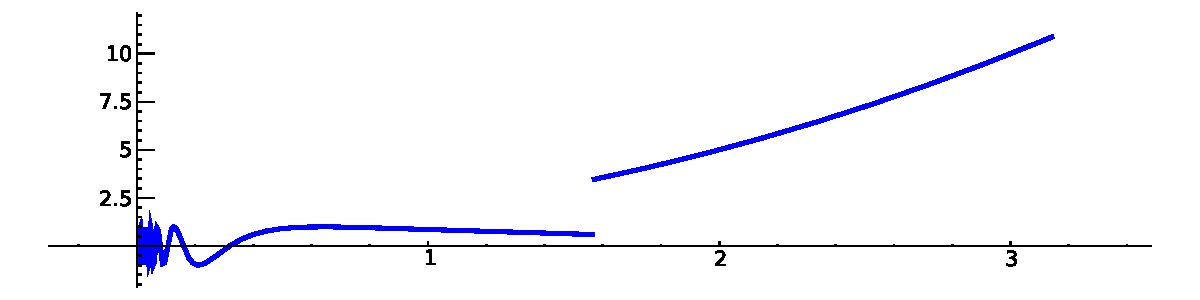
\includegraphics[width=25em]{piecewise.pdf}
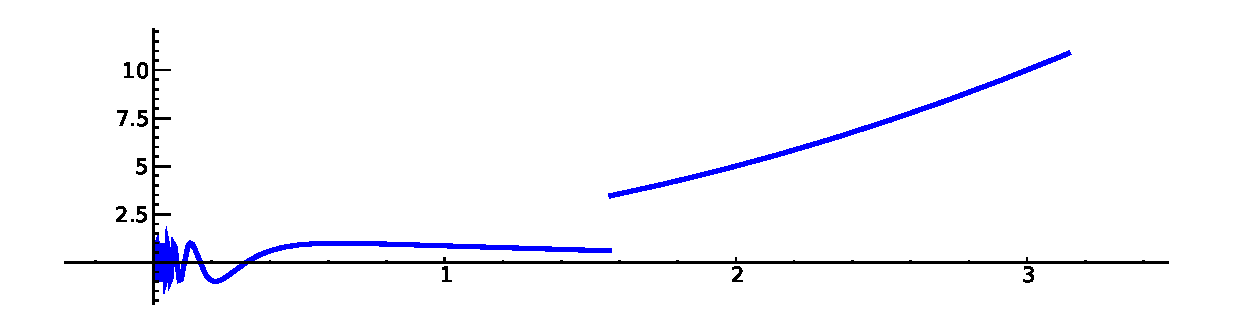
\includegraphics[width=25em]{piecewise.eps}

%*********************************************
 \hr\textbf{Python functions}

Defining:

{\ex\verb|def f(a, b, theta=1):|\\
\verb|    c = a + b*theta^2|\\
\verb|    return c|}

Inline functions:

{\ex\verb|    f = lambda a, b, theta = 1: a + b*theta^2|}

\vspace{.8em}

%*********************************************
\hr\textbf{Simplifying and expanding}

Below $f$ must be symbolic (so {\bf not} a Python function):

Simplify: \verb|f.simplify_exp()|, \verb|f.simplify_full()|,\\
\mbox{}\,\verb|        f.simplify_log()|, \verb|f.simplify_radical()|,\\
\mbox{}\,\verb|        f.simplify_rational()|, \verb|f.simplify_trig()|

Expand: \verb|f.expand()|, \verb|  f.expand_rational()|


%*********************************************
\hr\textbf{Equations}

Relations: $f=g$: \verb|f == g|, $f\neq g$: \verb|f != g|, \\
\mbox{}$\,\,\,\,\qquad\qquad f\leq g$: \verb|f <= g|, $f\geq g$: \verb|f >= g|, \\
\mbox{}$\,\,\,\,\qquad\qquad f< g$: \verb|f < g|, $\,\,\,f> g$: \verb|f > g| 

Solve $f=g$: \verb| solve(f == g, x)|, and\\
\verb|            solve([f == 0, g == 0], x,y)|

{\ex \verb|   solve([x^2+y^2==1, (x-1)^2+y^2==1],x,y)|}

Solutions: \\
{\ex \verb|  S = solve(x^2+x+1==0, x, solution_dict=True)|}\\
{\ex \verb|    S[0]["x"]   S[1]["x"]  |} are the solutions

Exact roots: {\ex \verb|  (x^3+2*x+1).roots(x)|}\\
Real roots: {\ex \verb|   (x^3+2*x+1).roots(x,ring=RR)|}\\
Complex roots: {\ex \verb|(x^3+2*x+1).roots(x,ring=CC)|}\\

%*********************************************
\hr\textbf{Factorization}

Factored form: {\ex \verb|(x^3-y^3).factor()|}\\
List of (factor, exponent) pairs:\\
{\ex\verb|(x^3-y^3).factor_list()|}

%*********************************************
\hr\textbf{Limits}

$\displaystyle\lim_{x\to a} f(x)=$ \verb|limit(f(x), x=a)|

{\ex\verb|   limit(sin(x)/x, x=0)|}

$\displaystyle\lim_{x\to a^+} f(x)=$ \verb|limit(f(x), x=a, dir='plus')|

{\ex\verb|   limit(1/x, x=0, dir='plus')|}

$\displaystyle\lim_{x\to a^-} f(x)=$ \verb|limit(f(x), x=a, dir='minus')|

{\ex\verb|   limit(1/x, x=0, dir='minus')|}



%*********************************************
\hr\textbf{Derivatives}

$\frac{d}{dx}(f(x))=$ \verb|diff(f(x),x) = f.diff(x)|

$\frac{\partial}{\partial x}(f(x,y))=$ \verb|diff(f(x,y),x)|

\verb|diff| $=$ \verb|differentiate| $=$ \verb|derivative|

{\ex\verb|   diff(x*y + sin(x^2) + e^(-x), x)|}

\vspace{2em}

%*********************************************
\hr\textbf{Integrals}

$\int f(x)dx=$ \verb|integral(f,x) = f.integrate(x)|

{\ex \verb|   integral(x*cos(x^2), x)|}

$\int_a^b f(x)dx=$ \verb|integral(f,x,a,b)|

{\ex \verb|   integral(x*cos(x^2), x, 0, sqrt(pi))|}

$\int_a^b f(x)dx \approx$ \verb|numerical_integral(f(x),a,b)[0]|

{\ex \verb|   numerical_integral(x*cos(x^2),0,1)[0]|}

\verb|assume(...)|: use if integration asks a question

   {\ex \verb|   assume(x>0)|}

%\mbox{}\,\quad([0] gives integral and [1] gives error bound)

%*********************************************
\hr\textbf{Taylor and partial fraction expansion}

Taylor polynomial, deg $n$ about $a$:\\
\verb|taylor(f,x,a,n)|$\approx c_0 + c_1(x-a) + \cdots + c_n(x-a)^n$

{\ex\verb|   taylor(sqrt(x+1), x, 0, 5)|}

Partial fraction:

{\ex \verb|(x^2/(x+1)^3).partial_fraction()|}


%*********************************************
\hr\textbf{Numerical roots and optimization}

Numerical root: \verb|f.find_root(a, b, x)|\\
{\ex \verb|   (x^2 - 2).find_root(1,2,x)|}\\
Maximize: find $(m,x_0)$ with $f(x_0)=m$ maximal\\
\verb|    f.find_maximum_on_interval(a, b, x)|\\
Minimize: find $(m,x_0)$ with $f(x_0)=m$ minimal\\
\verb|    f.find_minimum_on_interval(a, b, x)|

Minimization: \texttt{minimize(f, {\it start\_point})}\\
{\ex\verb|   minimize(x^2+x*y^3+(1-z)^2-1, [1,1,1])|}

%*********************************************
\hr\textbf{Multivariable calculus}

Gradient: \verb|f.gradient()| or \texttt{f.gradient({\it vars})}\\
{\ex \verb|    (x^2+y^2).gradient([x,y])|}

Hessian: \verb|f.hessian()|\\
{\ex \verb|    (x^2+y^2).hessian()|}

Jacobian matrix: \texttt{jacobian(f, {\it vars})}\\
{\ex \verb|    jacobian(x^2 - 2*x*y, (x,y))|}

%*********************************************
\hr\textbf{Summing infinite series}

$$\sum_{n=1}^{\infty} \frac{1}{n^2} = \frac{\pi^2}{6}$$

{\em Not yet implemented, but you can use Maxima:}\\
{\ex\verb|s = 'sum (1/n^2,n,1,inf), simpsum'|\\
\verb|SR(sage.calculus.calculus.maxima(s))|}
$\longrightarrow \pi^2/6$



\end{multicols*}

\end{document}
